\section{Ejecucion grafica y por consola}
\begin{itemize}
  \item A continuacion se vera la Ejecucion tanto grafica como por consola
\end{itemize}
\subsection{Ejecucion por consola}
\begin{lstlisting}
===== Ejercito 1 =====
 Soldado 0x8:
  Nivel de vida: 3
  Fila: 9
  Columna: 2

 Soldado 0x6:
  Nivel de vida: 3
  Fila: 3
  Columna: 1

 Soldado 0x7:
  Nivel de vida: 5
  Fila: 1
  Columna: 1

 Soldado 0x4:
  Nivel de vida: 4
  Fila: 2
  Columna: 2

 Soldado 0x5:
  Nivel de vida: 1
  Fila: 6
  Columna: 3

 Soldado 0x2:
  Nivel de vida: 4
  Fila: 4
  Columna: 6

 Soldado 0x3:
  Nivel de vida: 3
  Fila: 10
  Columna: 1

 Soldado 0x0:
  Nivel de vida: 4
  Fila: 2
  Columna: 6

 Soldado 0x1:
  Nivel de vida: 2
  Fila: 3
  Columna: 3


===== Ejercito 2 =====
 Soldado 1x3:
  Nivel de vida: 1
  Fila: 1
  Columna: 4

 Soldado 1x1:
  Nivel de vida: 3
  Fila: 5
  Columna: 3

 Soldado 1x2:
  Nivel de vida: 4
  Fila: 3
  Columna: 9

 Soldado 1x0:
  Nivel de vida: 1
  Fila: 6
  Columna: 5

Soldado con maxima vida:
 Soldado 0x7:
  Nivel de vida: 5
  Fila: 1
  Columna: 1


===== Ranking de soldados: =====
 Soldado 0x7:
  Nivel de vida: 5
  Fila: 1
  Columna: 1

 Soldado 0x2:
  Nivel de vida: 4
  Fila: 4
  Columna: 6

 Soldado 1x2:
  Nivel de vida: 4
  Fila: 3
  Columna: 9

 Soldado 0x0:
  Nivel de vida: 4
  Fila: 2
  Columna: 6

 Soldado 0x4:
  Nivel de vida: 4
  Fila: 2
  Columna: 2

 Soldado 1x1:
  Nivel de vida: 3
  Fila: 5
  Columna: 3

 Soldado 0x8:
  Nivel de vida: 3
  Fila: 9
  Columna: 2

 Soldado 0x6:
  Nivel de vida: 3
  Fila: 3
  Columna: 1

 Soldado 0x3:
  Nivel de vida: 3
  Fila: 10
  Columna: 1

 Soldado 0x1:
  Nivel de vida: 2
  Fila: 3
  Columna: 3

 Soldado 1x3:
  Nivel de vida: 1
  Fila: 1
  Columna: 4

 Soldado 0x5:
  Nivel de vida: 1
  Fila: 6
  Columna: 3

 Soldado 1x0:
  Nivel de vida: 1
  Fila: 6
  Columna: 5
\end{lstlisting}
\begin{itemize}
  \item Como vemos, la estructura del metodo main esta representada en la salida por consola
  \item A continuacion se vera la salida grafica:
\end{itemize}
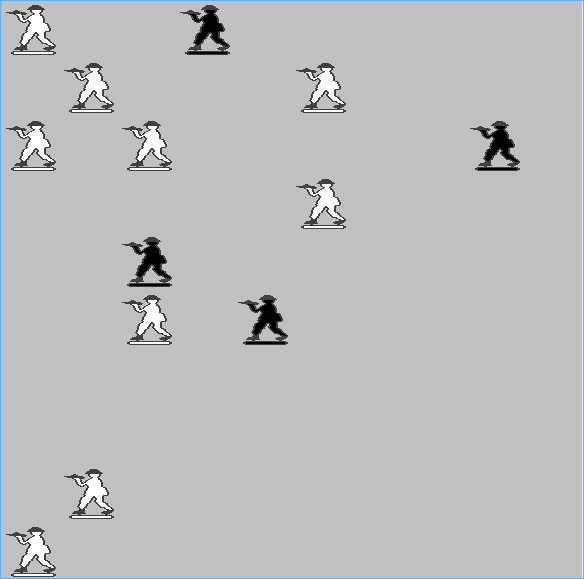
\includegraphics[width=0.5\textwidth]{img/exec.png}
